The model of decay time and decay angles in the \BstoJpsiKK{} decay, as presented in Chapters~\ref{chap:pheno} and \ref{chap:ana}, is
fitted to the data from reconstructed and selected $\Bs$ and $\Bsbar$ candidates, after background subtraction. Statistical uncertainties
in the resulting parameter estimates are evaluated from the shape of the likelihood function, as described in Chapter~\ref{chap:ana}.
Systematic uncertainties are estimated by repeating the fit with variations of the model or the data.

Results are presented for three different parameterizations of CP violation. Different assumptions are made, based on the conjectures that
the \BstoJpsiKK{} decay is dominated by a tree-level amplitude and that CP violation in mixing is small, as discussed in
Section~\ref{subsec:intro_Jpsiphi_decay}. If contributions from additional decay amplitudes are small, CP violation is induced by the
\BsBsbar{} mixing process and does not depend on the intermediate state. Also CP violation in decay will be small in this case.

The first parameterization is the most general one and includes different parameters $\phisi$ and $\Csi$ for the intermediate states
$i\in\{\text{0}, \parallel, \perp, \text{S}\}$. See Section~\ref{subsec:pheno_equations_param} for a description of the actual parameters
that are used. The second parameterization is more restrictive and assumes that CP-violating effects are identical among the intermediate
states. Finally, for the third parameterization the additional assumptions of no CP violation in mixing and no CP-violation in decay are
made. The following parameters describe CP violation for these three cases:
\begin{enumerate}
  \item $\phisav,\Delphispara,\Delphisperpp,\DelphisS
         \quad\text{and}\quad\Csav,\DelCspara,\DelCsperp,\CsavS$
  \item $\phisi[\text{0}]=\phisi[\parallel]=\phisi[\perp]=\phisi[\text{S}]\equiv\phis
         \quad\text{and}\quad\lamsiAbs[\text{0}]=\lamsiAbs[\parallel]=\lamsiAbs[\perp]=\lamsiAbs[\text{S}]\equiv\lamsAbs$
  \item $\phisi[\text{0}]=\phisi[\parallel]=\phisi[\perp]=\phisi[\text{S}]\equiv\phis
         \quad\text{and}\quad\lamsiAbs[\text{0}]=\lamsiAbs[\parallel]=\lamsiAbs[\perp]=\lamsiAbs[\text{S}]\equiv1$
\end{enumerate}

Figures~\ref{fig:timeProjections} and \ref{fig:angleProjections} show the background-subtracted distributions of decays in time and angles
and the corresponding one-dimensional PDF projections for case 2, the $\phis$/$\lamsAbs$ model. The decay-time distribution is shown in
both the full selected range of [0.3, 14]~ps on a logarithmic vertical scale (Figure~\ref{fig:timeProjections_log}) and in a reduced range
of [0.3, 5]~ps on a linear vertical scale (Figure~\ref{fig:timeProjections_lin}).
\begin{figure}[htb]
  \centering
  \begin{subfigure}{0.49\textwidth}
    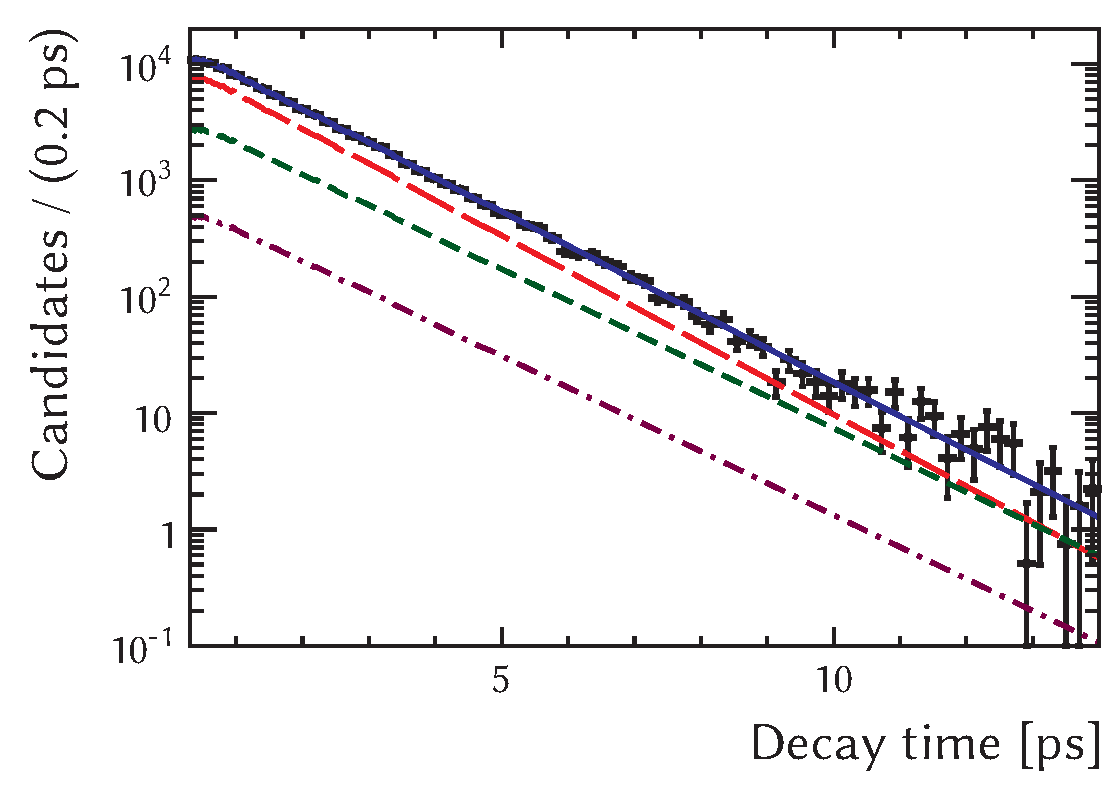
\includegraphics[width=\textwidth]{graphics/results/timeLog}
    \caption{}
    \label{fig:timeProjections_log}
  \end{subfigure}
  \hfill%
  \begin{subfigure}{0.49\textwidth}
    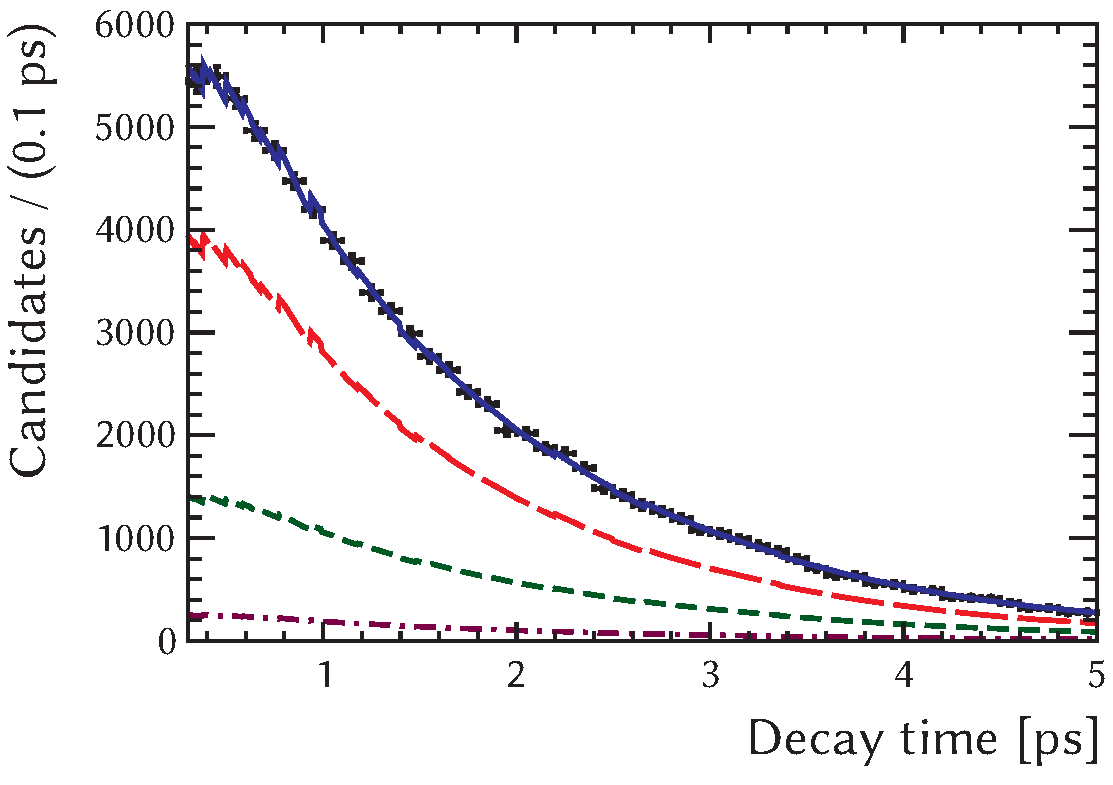
\includegraphics[width=\textwidth]{graphics/results/timeLin}
    \caption{}
    \label{fig:timeProjections_lin}
  \end{subfigure}

  \caption{Background-subtracted distribution of decays in decay time (data points)
           and the corresponding one-dimensional projection of the PDF (blue line).
           Figure~(a) shows the distribution in the full range between 0.3 and 14\unitsp{}ps
           on a logarithmic vertical scale, while Figure~(b) shows the distribution between 0.3 and 5\unitsp{}ps
           on a linear vertical scale.
           Additional PDF projections are shown for the CP-even (long-dashed, red line) and CP-odd (short-dashed, green line)
           components of \BstoJpsiphi{} and for the S-wave (dashed-dotted, magenta line).}
  \label{fig:timeProjections}
\end{figure}
%
\begin{figure}[htbp]
  \centering
  \begin{subfigure}{0.49\textwidth}
    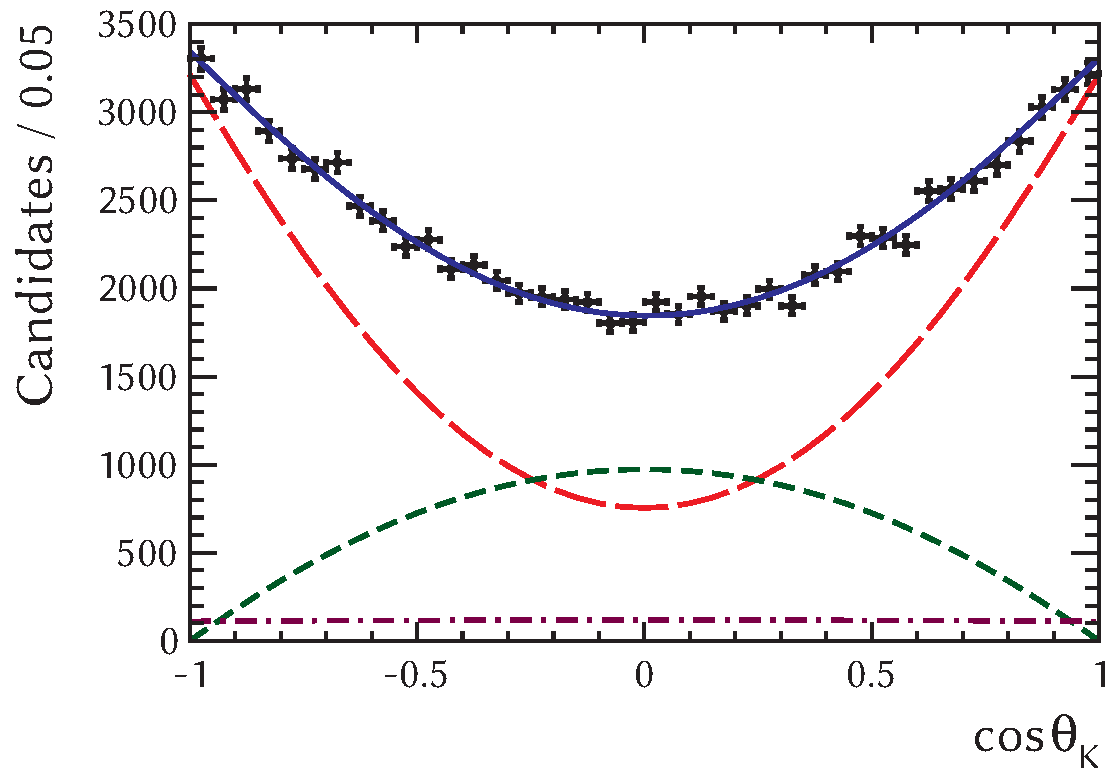
\includegraphics[width=\textwidth]{graphics/results/ctk}
    \caption{}
  \end{subfigure}
  \hfill%
  \begin{subfigure}{0.49\textwidth}
    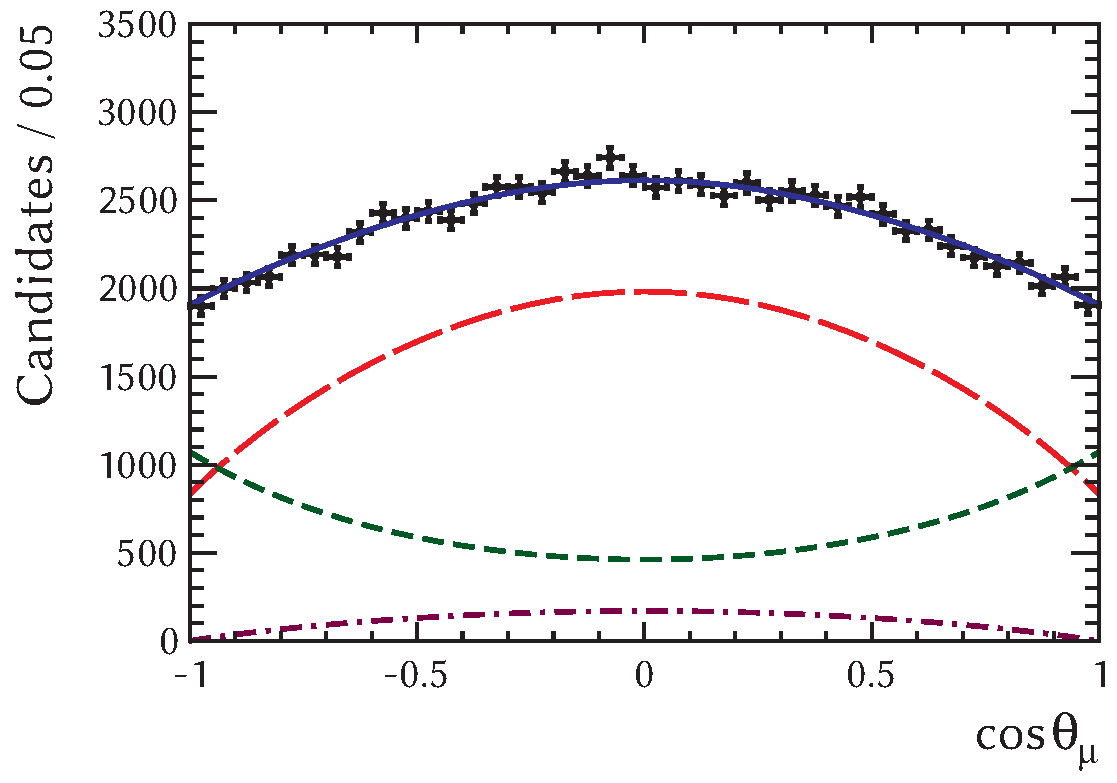
\includegraphics[width=\textwidth]{graphics/results/ctl}
    \caption{}
  \end{subfigure}

  \vspace*{0.02\textwidth}
  \begin{subfigure}{0.49\textwidth}
    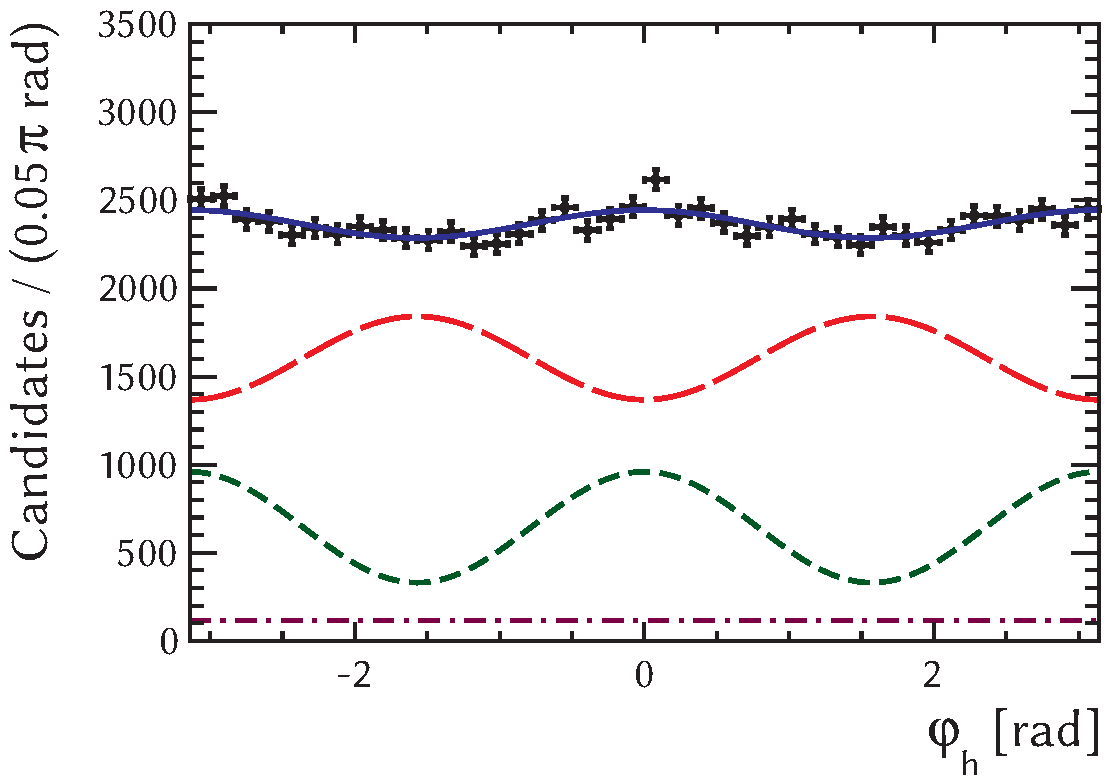
\includegraphics[width=\textwidth]{graphics/results/phi}
    \caption{}
  \end{subfigure}

  \caption{Background-subtracted distribution of decays in decay angles (data points)
           and the corresponding one-dimensional projections of the PDF (solid, blue line).
           The distributions of $\cthetaK$, $\cthetal$, and $\phihel$ are shown in Figures~(a), (b), and (c), respectively.
           Additional PDF projections are shown for the CP-even (long-dashed, red line) and CP-odd (short-dashed, green line)
           components of \BstoJpsiphi{} and for the S-wave (dashed-dotted, magenta line).}
  \label{fig:angleProjections}
\end{figure}

The solid, blue lines in Figures~\ref{fig:timeProjections} and \ref{fig:angleProjections} represent the projections of the full PDF and are
to be compared to the distributions of the data. In addition, the contributions of CP-even and CP-odd intermediate states to the PDF are
shown separately. The long-dashed, red lines represent the sum of the $\magzeroSq$ and $\magparSq$ terms in the PDF, which are CP even. The
CP-odd $\magperpSq$ and $\magSSq$ terms are shown as the short-dashed, green and dashed-dotted, magenta lines, respectively. Contributions
from interference terms are not shown. The discontinuities in the decay-time PDFs arise from statistical uncertainties in the bin
coefficients of the acceptance function.

Even though the angular dependence of the interference terms is not visible in the projection plots, they clearly show differences in the
shapes of the CP-even and CP-odd components, which enable a statistical separation. In $\cthetaK$ and $\cthetal$ the difference between
the even and odd \BstoJpsiphi{} components is made by the $\magzeroSq$ and $\magperpSq$ angular functions. Where the $\magzeroSq$ term has
a $\cos^2\theta$ behaviour, the $\magperpSq$ term has a $\sin^2\theta$ behaviour and vice versa. In $\phihel$ the $\magzeroSq$ function is
uniform, but the oscillatory behaviour for $\magparSq$ is opposite to that of the $\magperpSq$ function. The $\KK$ S-wave term is uniform
in $\cthetaK$ and $\phihel$, but proportional to $\sin^2\thetal$.

The largest contribution to the \BstoJpsiphi{} decay rate comes from the CP-even $\magzeroSq$ and $\magparSq$ components, which account for
approximately 75\%. Although this cannot be seen in these projection plots, $\magparSq$ and $\magperpSq$ are roughly equal. The S-wave
accounts for approximately 5\% of the total.

From the decay-time plot with logarithmic vertical scale it is clear that the CP-even intermediate states decay faster than the CP-odd
intermediate states. In case CP violation is small, the even states roughly correspond to the light CP eigenstate of the \BsBsbar{} system
and the odd states to the heavy CP eigenstate (Equation~\ref{eq:timeCPEvenOdd}). Under this assumption it can be inferred from the
lifetimes of the states that the decay width of the light state is larger and hence that $\DGs\equiv\GL-\GH$ is positive.

The plots in Figure~\ref{fig:timeProjections} show the sum of the $\Bs$ and $\Bsbar$ decay-time distributions, for which the decay-time
oscillation vanishes. Since most of the sensitivity for the CP-violation parameters comes from the amplitudes of the oscillation terms,
these projection plots contain little information on the CP-violation measurement. More information is contained in
Figure~\ref{fig:BBbarAsymmetry}, which shows the asymmetry between $\Bs$ tags and $\Bsbar$ tags.
\begin{figure}[htb]
  \centering
  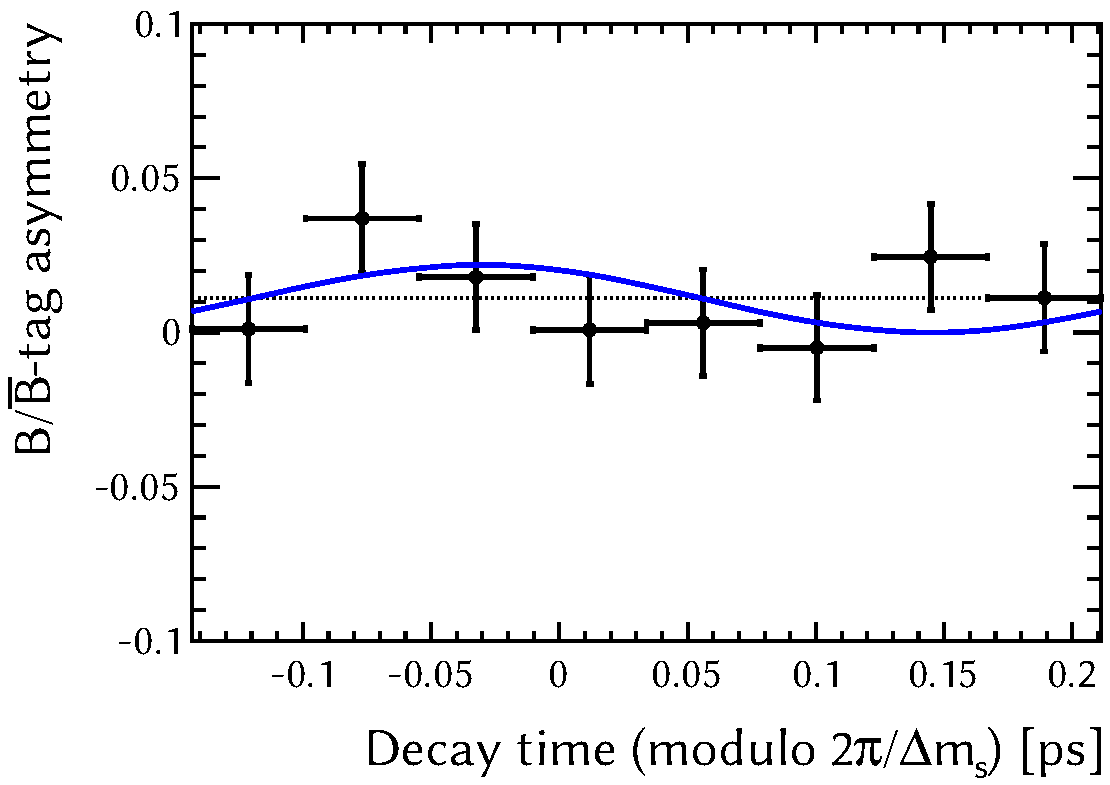
\includegraphics[width=0.75\textwidth]{graphics/results/asym}
  \caption{Background-subtracted asymmetry in the numbers of decays with $\Bs$ and with $\Bsbar$ flavour tags as a function of decay time
           (data points) and the corresponding asymmetries in the PDFs for the $\phisi$/$\Csi$ (solid, blue line),
           $\phis$/$\lamsAbs$ (dashed-dotted, green line), and $\phis$/$\lamsAbs$\texteq1 (dashed, red line) parameterizations.
           Data from the full decay-time range are mapped onto one period of the expected oscillation in the asymmetry.
           Decay candidates are weighted by the product of the corresponding estimated dilution factors from decay-time resolution
           and wrong tags to optimize the significance of the displayed asymmetry.}
  \label{fig:BBbarAsymmetry}
\end{figure}

The \BsBsbar-tag asymmetry is defined as
\[
  A_{\text{tag}} \equiv \frac{\#\Bs{}\text{ tags} - \#\Bsbar{}\text{ tags}}{\#\Bs{}\text{ tags} + \#\Bsbar{}\text{ tags}}
\]
and is shown in bins of decay-time for the background-subtracted data. The corresponding asymmetry in the PDFs for $\Bs$ tags and $\Bsbar$
tags at each point in decay time is shown for the three parameterizations by the lines in the figure. The data asymmetry in a bin is
predicted by the mean of the PDF asymmetry in that bin. An oscillation can be observed in the asymmetry as a function of decay time
provided that CP symmetry is violated (Equation~\ref{eq:timeOscill}) and that the dilution factors from flavour tagging and decay-time
resolution are non-zero.

To increase the statistical significance of the displayed asymmetry in the data all oscillation periods are projected onto the one period
of approximately 0.36\unitsp{}ps that is shown in Figure~\ref{fig:BBbarAsymmetry}. This period starts at about \tm0.06\unitsp{}ps, onto
which the lower edge of the decay-time range in the analysis of 0.3\unitsp{}ps is mapped.

The significance of the displayed oscillation is further enhanced by the use of flavour-tagging and decay-time resolution information.
The amplitude of the oscillation in the plot is maximized with respect to its uncertainty by weighting the contribution of each decay
candidate by the product of the corresponding dilution factors from tagging and resolution.

With the assumption $\lamsAbs$\texteq{}1 the cosine component of the PDF vanishes. This can be seen in the figure, which shows a sine
function for the $\phis$/$\lamsAbs$\texteq{}1 parameterization (dashed, red line). The function has a negative slope at zero decay-time,
which indicates a negative value of $\phis$, assuming the CP-even components dominate the decay (see Equation~\ref{eq:timeOscill}). The
function for the $\phisi$/$\Csi$ parameterization (solid, blue line) almost overlaps with the $\phis$/$\lamsAbs$\texteq{}1 function. This
indicates that the $\Csi$ parameter values are small or that they effectively cancel, resulting in a vanishing cosine component.

The oscillation for the $\phis$/$\lamsAbs$ parameterization can be described as a negative sine function with a phase offset of about
0.055\unitsp{}ps\textcdot$\Dms$\textapprox0.31$\,\pi$\unitsp{}rad (dashed-dotted, green line in Figure~\ref{fig:BBbarAsymmetry}), implying
that both the sine and the cosine coefficients in Equation~\ref{eq:timeOscill} have non-zero values for this parameterization. The
contribution of the cosine also makes the amplitude of the oscillation larger than the amplitudes for the other two parameterizations. With
this phase offset the magnitude of the cosine coefficient is roughly a factor 1.5 larger than the magnitude of the sine coefficient. The
latter coefficient is again negative, which implies a negative value for $\phisav$.

Despite the fact that the asymmetry plot shows an oscillation in the $\Bs$ and $\Bsbar$ PDFs, the statistical uncertainties on the data
points show that this oscillation is not significant. This indicates that that the estimates of the $\phis$ and $\Cs$ from the fit also do
not differ from zero significantly.

Also the overall mean \BsBsbar-tag asymmetry in the data, indicated by the dotted, black line, is not statistically significant. A non-zero
mean could arise from production and tagging asymmetries. The PDFs for $\Bs$ tags and $\Bsbar$ tags are weighted by the number of decays in
the corresponding category, which makes the mean asymmetry in the PDF equal to the value in the data by construction.
